\documentclass[12pt]{article}

\usepackage[a4paper, margin=1in]{geometry} % Margins
\usepackage{fancyhdr} % Set header and footer
\usepackage{titling}

\usepackage[T1]{fontenc} % For international characters
\usepackage{XCharter} % XCharter as the main font

\usepackage[
  backend=biber,
  style=numeric,
  citestyle=authoryear,
  sorting=none
  ]{biblatex}
\addbibresource{./Ref/reference.bib}

\usepackage[english]{babel} % Use english by default
\usepackage{csquotes}

\usepackage{amsmath, amsthm, amssymb, amsfonts, mathtools}
\usepackage{graphicx}
\usepackage{tikz}
\usetikzlibrary{shapes, arrows}
% \usepackage[]{algorithm2e}
% \usepackage{caption, enumerate}
% \usetikzlibrary{graphdrawing, shapes}
% \usegdlibrary{trees}

\usepackage{hyperref}
\hypersetup{
  colorlinks,
  citecolor=black,
  filecolor=black,
  linkcolor=black,
  urlcolor=black
}

\pagestyle{fancy}
\fancyhf{}
\fancyhead[R]{Leo W.}
\fancyfoot[R]{\thepage}
\setlength{\headheight}{15pt}

%----------------------------------------------------------------------------------------
%	CUSTOM COMMANDS
%----------------------------------------------------------------------------------------

\newcommand{\articletitle}[1]{\renewcommand{\articletitle}{#1}} % Define a command for storing the article title
\newcommand{\articlecitation}[1]{\renewcommand{\articlecitation}{#1}} % Define a command for storing the article citation
\newcommand{\doctitle}{\articlecitation\ --- ``\articletitle''} % Define a command to store the article information as it will appear in the title and header
\newcommand{\doctitlenocite}{\articletitle} % No citation

\newcommand{\datenotesstarted}[1]{\renewcommand{\datenotesstarted}{#1}} % Define a command to store the date when notes were first made
\newcommand{\docdate}[1]{\renewcommand{\docdate}{#1}} % Define a command to store the date line in the title

\newcommand{\docauthor}[1]{\renewcommand{\docauthor}{#1}} % Define a command for storing the article notes author

\newcommand{\bookcitation}[1]{\renewcommand{\bookcitation}{#1}} % Define a command for storing the book citation

% Define a command for the structure of the document title
\newcommand{\printtitle}{
\begin{center}
\textbf{\Large{\doctitle}}

\docdate

\docauthor
\end{center}
}

% No citation
\newcommand{\printtitlenocite}{
\begin{center}
\textbf{\Large{\doctitlenocite}}

\docauthor

\docdate
\end{center}
}

%----------------------------------------------------------------------------------------
%	STRUCTURE MODIFICATIONS
%----------------------------------------------------------------------------------------

\setlength{\parskip}{3pt} % Slightly increase spacing between paragraphs

% Uncomment to center section titles
% \usepackage{sectsty}
% \sectionfont{\centering}

% Uncomment for Roman numerals for section numbers
% \renewcommand\thesection{\Roman{section}}
% \renewcommand\thesubsection{\thesection.\Roman{subsection}}


\title{Introductory Backtesting Notes \\ for Quantitative Trading Strategies \\[2ex]
  \large Useful Metrics and Common Pitfalls}
\author{Leo Wong (QFIN \& COSC, HKUST)}
\date{December, 2019}

\begin{document}

\begin{titlingpage}
  \maketitle
  \begin{abstract}
    This note is compiled for COMP4971C in Fall 2019 to assist the research and implementation of quantitative trading strategies. This note includes suggested evaluation metrics and common pitfalls for beginners in quantitative trading and backtest.

    It is common nowadays to use mathematical and statistical models to evalute financial securities and take corresponding actions. However, attention to details is one of the crucial factors to make a strategy successful in reality, when various academic assumptions do not hold. Having proper assumptions and configuration for backtest may cover more situations and provide more robust evaluation of trading strategies. Thus, it enhances the quality of trading strategies as the backtest provides more realistic results and more accurate approximations.

    \enquote{All models are wrong, but some are useful}, \cite{allmodelsarewrong}.
  \end{abstract}
\end{titlingpage}

\fancyhead[L]{Introductory Backtesting Notes}

\tableofcontents

\section{Introduction}

Backtesting is a compulsory stage in the development of any quantitative trading strategies. It evaluates the performance of a strategy with historical data and provides the following usages:

\begin{enumerate}
  \item validate the effectiveness of the trading idea
  \item tune the parameters of the strategy
  \item predict the future performance (assuming repeating market patterns)
\end{enumerate}

This note briefly introduces some industrial practices in backtesting a quantitative trading strategy for general first order securities (e.g. equity share, commodity future, etc.) along with some common mistakes. The majority of the content comes from several books and articles including but not limited to \cite{insideblackbox}, \cite{succalgotrading}, \cite{epchan2008}. All references are listed at the end of the note.

The structure diagram of a suggested backtest system is included below.

\tikzset{%
  block/.style    = {draw, thick, rectangle, minimum height = 3em, minimum width = 3em},
  sum/.style      = {draw, circle, node distance = 2cm}, % Adder
  input/.style    = {coordinate}, % Input
  output/.style   = {coordinate} % Output
}
% Defining string as labels of certain blocks.
\newcommand{\suma}{\Large$+$}
\newcommand{\inte}{$\displaystyle \int$}
\newcommand{\derv}{\huge$\frac{d}{dt}$}

\begin{tikzpicture}[auto, thick, node distance=2cm, >=triangle 45]
  \node at (2, 11) {\textsc{\large Structure of Backtest System}};
  \draw [thick] (1, 0) rectangle (13, 10);

  \draw node at (-1, 5) [block, name=data] {Data};
  \draw node at (3, 8) [block, name=alpha] {Alpha Model};
  \draw node at (6, 8) [block, name=risk] {Risk Model};
  \draw node at (10, 8) [block, name=cost] {Transaction Cost Model};
  \draw node at (7, 5) [block, name=portfolio] {Portfolio Construction Engine};
  \draw node at (7, 2) [block, name=execution] {Execution Engine};

  \draw[->] (data) -- (1, 5);
  \draw[->] (alpha) -- (portfolio);
  \draw[->] (risk) -- (portfolio);
  \draw[->] (cost) -- (portfolio);
  \draw[<->] (portfolio) -- (execution);

\end{tikzpicture}

\section{Note and Assumption}

\begin{enumerate}
  \item All \enquote{suggested} values are annualized, calculations are stated below
  \item All \enquote{suggested} values are calculated after deducting transaction cost
  \item Returns at different time \(t\) are assumed to be IID \footnote{Independent and identically distributed, i.e. assuming same probability distribution and mutually independent}, otherwise the estimation of Sharpe ratio from sample needs to be adjusted accordingly
\end{enumerate}

\section{Primary Metrics}

Primary metrics should be used for all types of trading strategies.

\subsection{Sharpe Ratio}

\subsubsection*{Metric Introduction}

Sharpe ratio is first introduced by \cite{sharpe1966}. Its original name \enquote{Reward-to-Variability Ratio} reflects its nature of balancing return and risk of a strategy. According to the definition in \cite{sharpe1994}, assume \(R_{Pt}\) as a \(t\)-period return series, \(R_{ft}\) as the risk-free rate series over the same period. Then the Sharpe ratio \(S_h\) from \(t=1\) to \(t=T\):

\begin{align*}
  S_h &\equiv \frac{\overline{D}}{\sigma_D} \\
  \text{where}~D &\equiv R_{Pt} - R_{ft} \\
  \overline{D} &\equiv \frac{1}{T} \sum_{t=1}^T D_t \\
  \sigma_D &\equiv \sqrt{\frac{\sum_{t=1}^T (D_t-\overline{D})^2}{T-1}}
\end{align*}

This Sharpe ratio indicates the historical average differential return per unit pf historical variability of the differential return (\cite{sharpe1966}). In simpler terms, Sharpe ratio measures the expected return gained per unit of risk taken for a zero investment strategy. The Sharpe ratio does not cover cases in which only one investment return is involved (\cite{sharpe1994}).

\subsubsection*{Suggested Level}

\begin{figure}[h!]
  \centering
  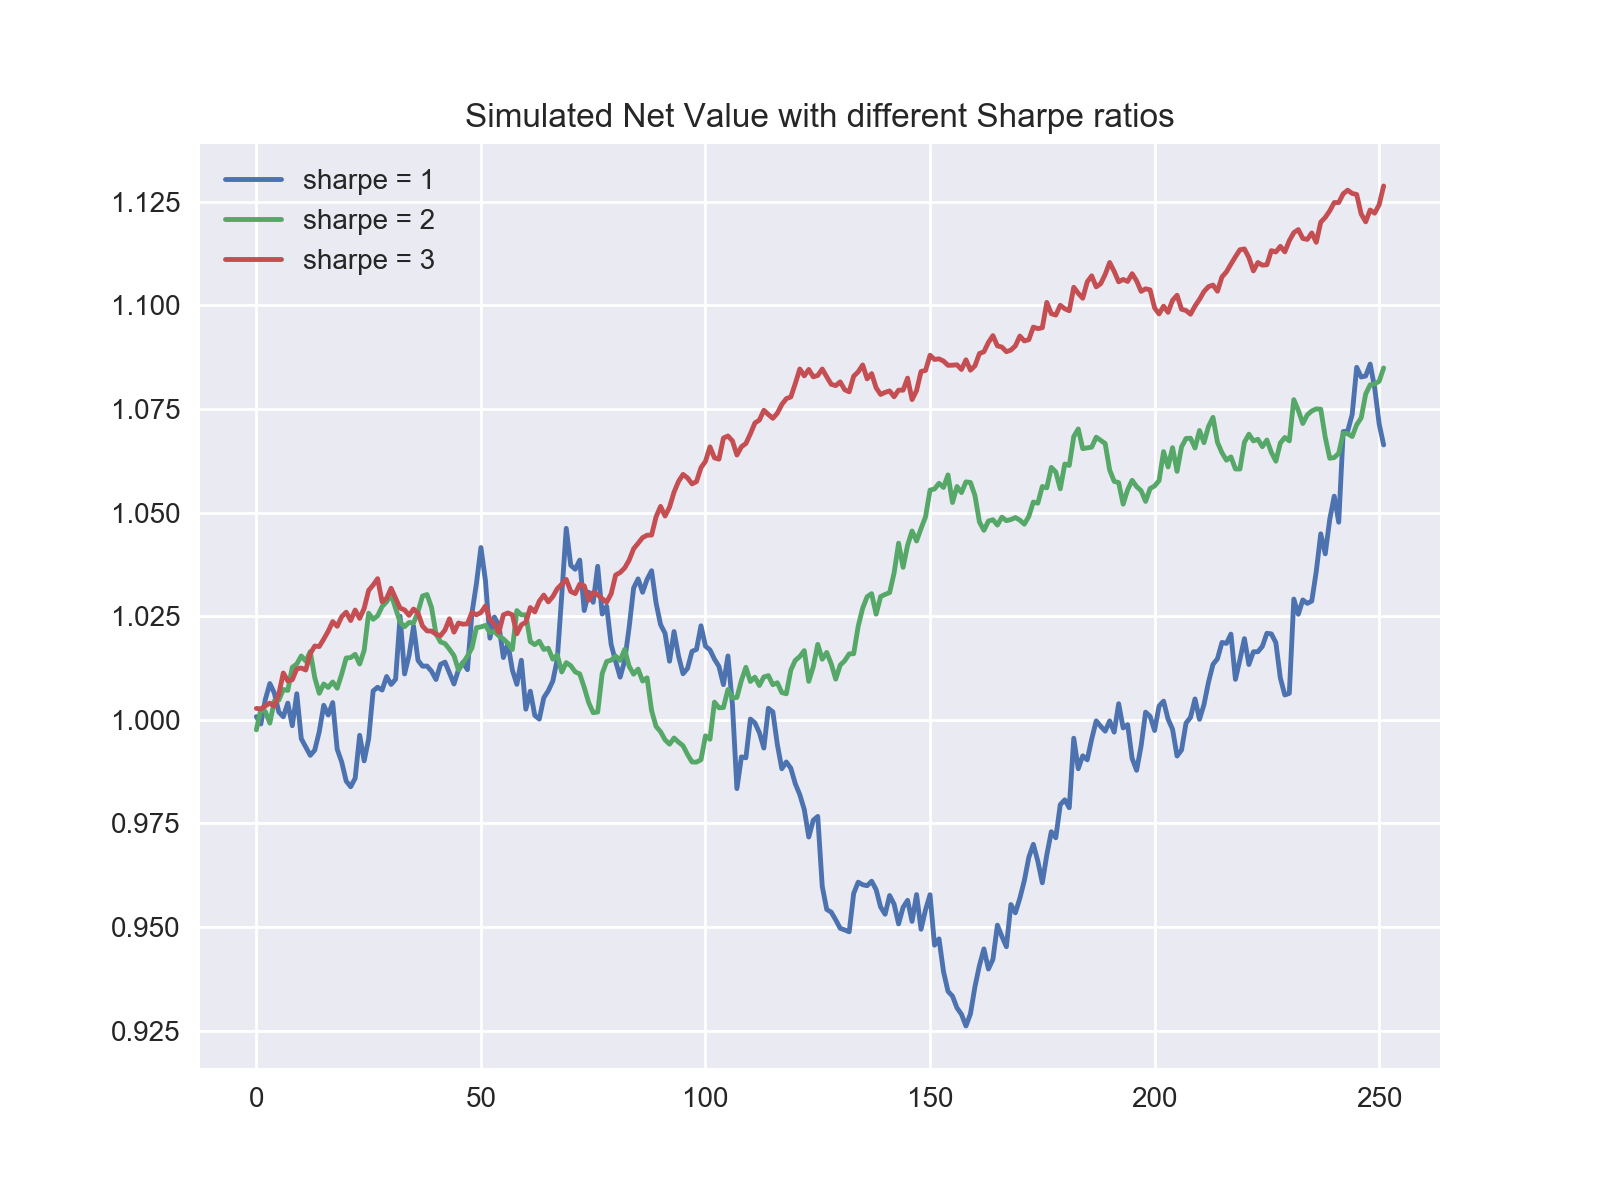
\includegraphics[scale=0.78]{./ref/figure/sharpe_nav_1200.png}
  \caption{Equity Curve of Multiple Sharpe Ratios}
  \label{fig:sharpe_navs}
\end{figure}

The above diagram shows 3 different return series of Sharpe ratios ranging from 1 to 3, with 252 steps (simulating year-long daily returns). For a day-frequency strategy, \(S_h > 1\) usually is not enough to generate consistent profits. A Sharpe value greater than 1.5 or even 2 is recommended. For longer-frequency strategies (i.e. weekly, monthly), \(S_h > 0.7\) can be acceptable, \(S_h > 1.2\) can be regarded as very good.

All values in the above section should be treated as reference instead of absolute limit/standard to judge a strategy.

\subsection{Maximum Drawdown}

\subsubsection*{Metric Introduction}

Maximum drawdown is a specific measure of drawdown (the peak-to-trough decline during a specified timespan) that measures the greatest decline from a peak, before a new peak is reached.

\begin{align*}
  MDD &= \min DD_i \tag*{where \(i \in {\{0, ..., T \}} \)} \\
  DD_t &= \frac{V_t}{\max \{V_0, V_1, ..., V_t \}}-1 \tag*{for \(t \in {\{0, ..., T \}} \)}
\end{align*}

Note that it only measures the size of the largest loss, not the frequency of large losses. MDD does not indicate how long it took an investor to recover from the loss, or if the investment even recovered at all.

\subsubsection*{Suggested Level}

\begin{figure}[h!]
  \centering
  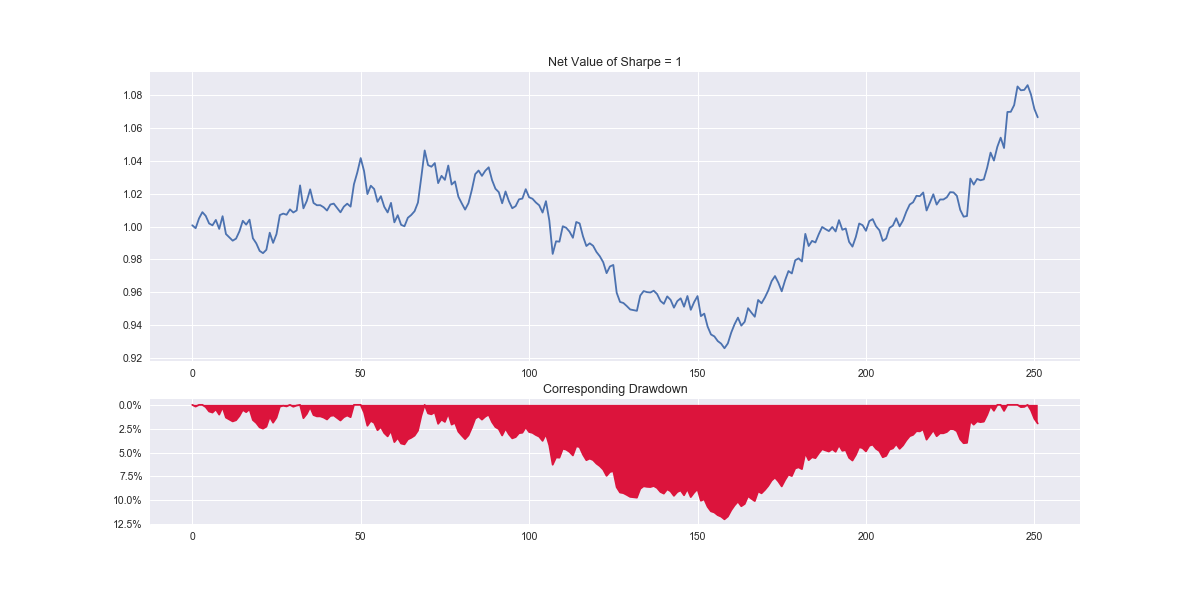
\includegraphics[scale=0.39]{./ref/figure/drawdown_nav_600.png}
  \caption{Equity Curve and Drawdown Graph}
  \label{fig:drawdown}
\end{figure}

The above diagram shows the net value and corresponding drawdown throughout the investment timespan. As shown in the diagram, \(0\%\) drawdowns refer to new peaks, consistent drawdowns below 0 refer to continuous loss. The maximum drawdown is the largest loss relative to the most recent peak in the investment timespan.

\subsection{Win Rate, Profit Factor and Payoff Ratio}

\subsubsection*{Metric Introduction}

Let \(\pi_t\) be the profit/loss of a strategy at time \(t\), \(T\) be the total number of steps (timespan). Assume the profit/loss is non-zero at every time \(t\), i.e. \(n_{\pi=0} = 0\), then \(T = n_{\pi<0} + n_{\pi>0}\). Let \(w\) be the win rate, \(pf\) be the profit factor, \(pr\) be the payoff ratio.

\begin{align*}
  w &= \frac{pf}{pf+pr} \\
  \text{where}~w &\equiv \frac{n_{\pi>0}}{n_{\pi<0} + n_{\pi>0}} \\
  pf &\equiv \frac{\sum_{t, \pi_t>0} \pi_t}{\sum_{t, \pi_t<0} \pi_t} \\
  pr &\equiv \frac{\sum_{t, \pi_t>0} \pi_t}{\sum_{t, \pi_t<0} \pi_t} \cdot \frac{n_{\pi<0}}{n_{\pi>0}}
\end{align*}

Win rate is expressed as the ratio of profiting time to the total investment timespan. Profit factor is the ratio of the sum of winning trades and losing trades. Payoff ratio is the ratio of winning trades average to losing trades average.

\subsubsection*{Suggested Level}

Win rate and payoff ratio are determined by the strategy characteristics, for example bare momentum-based strategies are usually related with relatively lower win rates due to the price reversion nature in multiple short term periods. Profit factor is more deterministic due to its definition. Therefore, we should focus on the former two metrics while win rate being the more dominant factor.

As win rate reflects the profiting consistency of a strategy, a higher win rate is almost always preferred. Win rate below the $50\%$ mark requires higher payoff ratio to compensate, the opposite portion is fine with smaller profit margin. Many profitable strategies made by individuals have win rates around $45\%$ to $55\%$. Professional knowledge and optimisation is often required to go beyond the common band.

\section{Secondary Metrics}

Secondary metrics provide easy explanation for non-finance-heavy personnel.

\subsection{Compound Annual Growth Rate (CAGR)}

\subsubsection*{Metric Introduction}

Compound annual growth rate (CAGR) is the annualized, required rate of return for an investment to grow in timespan \(T\) (in years), assuming the intermediate profits are reinvested.

\begin{align*}
  CAGR = \bigg(\frac{V_T}{V_0} \bigg)^{\frac{1}{T}}-1
\end{align*}

CAGR is not the true rate of return, but rather a smoothed, representational figure, usually used for easier explanation and comparison.

\subsubsection*{Suggested Level}

The desired CAGR depends on the nature of the security and even its sector. Different types of securities (e.g. equity, fixed income, index, derivative) have different return characteristics. Equity-type securities generally have a higher CAGR while corresponding derivatives are even more volatile. The performance of fixed income products are more consistent over time.

Note that CAGR can be affected by the level of leverage. Let $I_0$ and $L_0$ be the amount of private capital and leverage (borrowed capital) at time $t=0$, $r$ be the interest rate. Assume a leverage ratio of $0.2$, i.e. $\frac{L_0}{I_0+L_0} = 0.2$. Then
\begin{align*}
  CAGR &= \bigg(\frac{V_T-L_0\times (1+r)^T}{I_0} \bigg)^{\frac{1}{T}}-1 \\
       &= \bigg(\frac{V_T-0.25I_0\times (1+r)^T}{I_0} \bigg)^{\frac{1}{T}}-1 \\
       &= \bigg(\frac{V_T}{I_0}-0.25(1+r)^T \bigg)^{\frac{1}{T}}-1
\end{align*}

Therefore, when comparing the CAGR of different strategies, the leverage level and cost should be kept the same.

\subsection{Volatility of Return}

\subsubsection*{Metric Introduction}

Volatility is a statistical measure of the dispersion of returns. Volatility is often measured as either the standard deviation or variance of returns. Given $r_1, r_2, \dots , r_t$ be the return series of a $t$-step timespan.

\begin{align*}
  \sigma_r = \sqrt\frac{\sum_{i=1}^t (r_i-\mu_r)^2}{t-1}
\end{align*}

In most cases, higher volatility reflects higher risk of the strategy or security. So investors should monitor the metric as a proxy of investment risk.

\subsubsection*{Suggested Level}

Investors will have their corresponding level of tolerance. One may not prefer frequent, large fluctuations of their asset value such as a retired person who just aim to keep his/her savings with minimal investment income to combat inflation. On the other hand, younger investor may be more aggressive as they are able to endure more risks. Thus, the level of risk tolerance should be tailored based on personal situation independently.


\section{Common Pitfall}

This section introduces multiple common mistakes made by quants in backtest.

\subsection{Survivorship Bias}

Survivorship bias may lead to significantly inflated strategy performance. It occurs when strategies are tested on datasets that only include securities which "survived" the whole test period but excluding those delisted during the meantime such as, technology stocks that went bankrupt after the dot-com boom in early 2000s, closed banks in the 2008 global financial crisis. Restricting the trading universe to "survived" companies introduces a survivorship bias based on their historical success.

We may mitigate survivorship bias in backtest with survivorship bias free datasets and/or more recent data. The former one includes information of delisted equities during the test period while it is likely that fewer stocks are delisting in a more recent, shorter time period.

\subsection{Transaction Costs}

It is very easy for beginners in quantitative trading to neglect or underestimate the impacts of transaction costs on strategies. Apart from the well-known broker commissions and fees, the bulk of overall transaction cost consists of slippage and market impact.

Slippage is the change in the price between the time a trader or a system decides to transact and the time when the order is actually at an exchange for execution. The more accurate the forecast, the more likely the security is going towards to the expected price as time passes. But the price move does not benefit the trader as he has not got his trade to the market. In addition to time, slippage is also a function of the volatility of the security. Greater volatility implies greater and more frequent price swings.

Market impact follows the basic economic principles of supply and demand and it is proportional to the size of the trade. Given the trade size is significant relative to the market, when it is a large buy order at market price, it is likely that the original supply of that security at market price is not sufficient to cover the order. As a result, the trader would need to pay more to buy the remaining positions. Same concepts apply to the sell order.

\subsection{Market Regime}

Most quantitative models are built with historical data that quants use past relationships and behavior to model the market and help predict the future. Therefore, when the market regime changes, biased models tend to collapse. For example, it was a strong, bull market right before the 2008 global financial crisis. If we use data from 2005 to 2007 only, we are prone to the massive downswing after the test period. Thus, it is important to select the input data and range when building models.

\begin{quote}
  The trend is your friend until it bends.
  \textit{The Market}
\end{quote}

\subsection{Look Ahead Bias}

Look ahead bias refers to the accidental introduction of future information which may inflate the strategy performance. If the test period ranges from $t=0$ to $t=T$, then any data from $t_{T+1}, t_{T+2}, t_{T+3}, \dots$ should not be included or referred.

One may avoid such a bias by carefully slicing data upto the design timespan before calculating any parameters such as, mean, standard deviation, maxima, minima, etc.

\subsection{Overfitting}

Overfitting occurs when parameters are optimised against the train dataset but the performance degrades substantially when applied to an unseen dataset. As statistical models are simultaneously trying to minimise both the bias error and the variance error in order to improve model accuracy, such a situation can lead to overfitting in models, as the training error can be substantially reduced by introducing models with more flexibility (variation). However, such models can perform extremely poorly on out-of-sample data since they were essentially “fit” to the in-sample data.

Overfitting can also appear on the trading strategies apart from statistical models. For example, we could optimise the Sharpe ratio by varying entry and exit thresholds. While this may improve profitability or minimise risk in the backtest, live performance is likely to vary and decrease as we may have overfit the optimisations to noise in the historical data.

Spliting train dataset into independent train-validation sets can help overcome this problem. Models are trained with the train set while parameters are optimised with the validation set. Lastly, evaluate the model effectiveness on unseen test sets. The independence of the three parts help improve the robustness of models and prevent overfitting.

\section*{Conclusion}

lorem

\renewcommand{\refname}{Reference} % Change the default bibliography title
\printbibliography

\end{document}
